\subsection{General Subspace Methods}
\label{sec:subspace_methods}

Consider a general linear system $Ax=b$ with $A \in \mathbb{R}^{n \times n}$. The main goal of a subspace based iterative method is to extract an approximate solution to such a system from a (lower dimensional) subspace of $\mathbb{R}^n$. Let $\mathcal{K}$ denote such a subspace of dimension $m$, containing all the approximate \textit{candidate solutions} for the system. In order to single out a desired candidate from this space, it is necessary to impose a number of constraints $m$ that such a solution needs to fulfill. Typically, those are $m$ (independent) orthogonality conditions, applied to the residual vector $r = Ax-b$. In other words, $r$ is required to be orthogonal to $m$ linearly independent vectors which define another subspace of $\mathcal{L}$ of dimension $m$ such that $r \perp \mathcal{L}$.

Thus a subspace method aims to find an approximate solution $\hat{x}\in \mathcal{K}$ such that $A\hat{x}-b \perp \mathcal{L}$. Because iterative methods usually want to exploit the knowledge of an initial guess $\iter[0]{x}$, the solution should be sought in the affine space $\iter[0]{x}+\mathcal{K}$ instead of the homogeneous vector space $\mathcal{K}$ \cite{saad_iterative_2003} and the problem reformulates to:
\begin{equation}
    \text{determine } \hat{x} \in \iter[0]{x}+\mathcal{K}\text{,}\;\;\text{  such that } A\hat{x}-b \perp \mathcal{L}
\end{equation}

\noindent If $\hat{x}$ is written in the form $\hat{x}=\iter[0]{x}+\delta$, and the initial residual $\iter[0]{r} = A\iter[0]{x}-b$, then the above condition becomes:
\begin{equation}
    \iter[0]{r} - A\delta \perp \mathcal{L}
\end{equation}

\noindent The implications of this condition are illustrated in Figure~\hyperref[fig:subspace]{\ref{fig:subspace}}, showing it results in a  newly obtained residual $\hat{r}$ orthogonal to $\mathcal{L}$. In general, subspace methods create a sequence of such projections, using a new pair of subspaces $\mathcal{K}$ and $\mathcal{L}$ in each step with $\iter[0]{x}$ being equal to the most recent approximation obtained from the previous projection.

\begin{figure}[h]
    \centering
    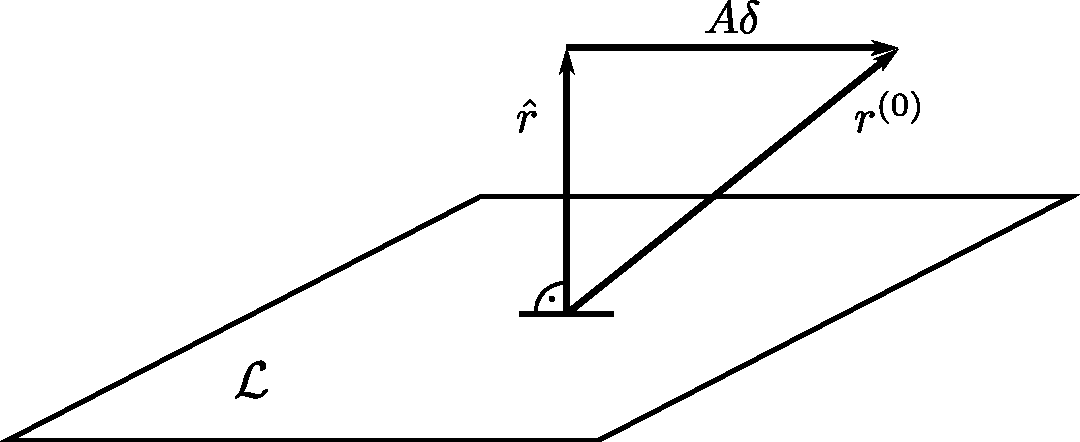
\includegraphics[width=0.7\linewidth]{chapters/2_solvers/2_3_iterative_solvers/figures/subspace.pdf}
    \caption{Interpretation of the orthogonality condition $\iter[0]{r} - A\delta \perp \mathcal{L}$ as described in \cite{saad_iterative_2003}}.
    \label{fig:subspace}
\end{figure}

\noindent This can also be expressed in matrix representation by defining a matrix $Q \in \realx{m}$, whose column vectors $Q =[q_1,\dots, q_m]$ form a basis of $\mathcal{K}$ and, similarly, a matrix $V \in \realx{m}$, whose column vectors $V = [v_q,\dots,v_m]$ form a basis of $\mathcal{L}$. The approximate solution is rewritten (with $y \in \real[m]$) as:
\begin{equation}
    \hat{x} = \iter[0]{x}+Vy
\end{equation}

\noindent From the orthogonality condition
\begin{equation}
    \iter[0]{r} -AVy \perp \mathcal{L}
\end{equation}

\noindent it follows that
\begin{equation}
    \transp{W}AVy = \transp{W}\iter[0]{r}
\end{equation}

\noindent and (if $\transp{W}AV$ is assumed to be non-singular)
\begin{equation}
    \hat{x} = \iter[0]{x}+V(\transp{W}AV)^{-1}\transp{W}\iter[0]{r}
\end{equation}

\noindent Since $\transp{W}AV$ is guaranteed to be non-singular, if no vector of the subspace $A\mathcal{K}$ is orthogonal to the subspace $\mathcal{L}$, \cite{saad_iterative_2003} lists two particular cases where this property is fulfilled:
\begin{enumerate}
    \item $A$ is positive definite and $\mathcal{L}=\mathcal{K}$, or
    \item $A$ is non-singular and $\mathcal{L}=A\mathcal{K}$
\end{enumerate}

\noindent The difference between these two cases is illustrated in Figure~\hyperref[fig:projection]{\ref{fig:projection}}, but before discussing them in detail, it is necessary to establish some basic properties of an orthogonal projection. If a vector $v$ is projected as vector $p$ into the subspace $\mathcal{K}$, then the deviation from the original vector is given by the error $e = v-p$. Let $P$ be the orthogonal projector onto the subspace $\mathcal{K}$ such that $p=Pv$ and $e\perp \mathcal{K}$ (as depicted in Figure~\hyperref[fig:subspace2]{\ref{fig:subspace2}}), then the length of $e$ is given by:
\begin{equation}
    \norm{v-p}_2 = \norm{v-Pv}_2
\end{equation}

\begin{figure}[h]
    \centering
    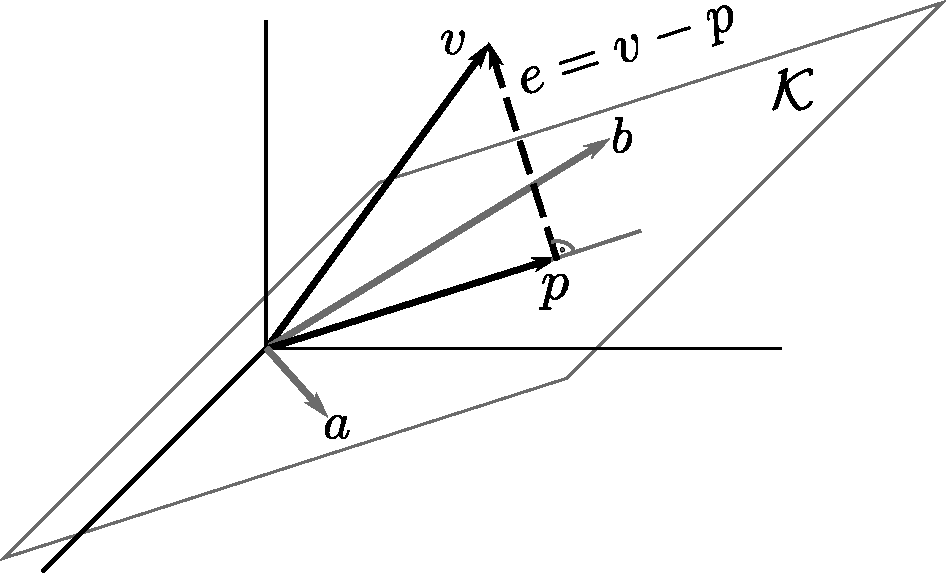
\includegraphics[width=0.7\linewidth]{chapters/2_solvers/2_3_iterative_solvers/figures/subspace2.pdf}
    \caption{Orthogonal projection $p$ of $v$ onto the subspace $\mathcal{K}$}.
    \label{fig:subspace2}
\end{figure}

\noindent Considering any other vectors $a,b \in \mathcal{K}$ with $a,b \neq p$ it follows that:
\begin{equation}
    \norm{v-a}_2>\norm{v-p}_2 \;\; \text{ and }\;\; \norm{v-b}_2>\norm{v-p}_2
\end{equation}

\noindent because (on the example of $a$):
\begin{equation}
    \norm{v-a}_1=\norm{x-Px}_2+\norm{Px-a}_2
\end{equation}

\noindent Therefore, it is established that the orthogonal projection process results in a vector $p \in \mathcal{K}$, that is closest to the original vector $v$ (i.e. that minimizes the error $\norm{e}_2$) \cite{strang_introduction_2009}. With this property in mind, the different choices for the subspace $\mathcal{L}$ (see Figure~\hyperref[fig:projection]{\ref{fig:projection}}) can be examined more carefully.

The second case, $\mathcal{L}=A\mathcal{K}$, is a little easier to interpret. It enforces the condition $A\hat{x}-b \perp A\mathcal{K}$, which is commonly referred to as the Petrov-Galerkin condition. This kind of projection where $\mathcal{K} \neq \mathcal{L}$ is called an oblique projection and can be seen in Figure~\hyperref[fig:projection_oblique]{\ref{fig:projection_oblique}}. In this case, the vector $A\delta$ is the orthogonal projection of the vector $\iter[0]{r}$ onto the subspace $A\mathcal{K}$, which guarantees that $\hat{r}$ will be minimal (as established in the previous paragraph). Consequently the residual can decrease (or stay constant) in each iteration and hence this kind of method is often called \textit{residual projection}.
\begin{equation}
    \norm{\hat{r}}\leq \normd{\iter[0]{r}}
\end{equation}

\begin{figure}
\centering
\begin{subfigure}{.5\textwidth}
  \centering
  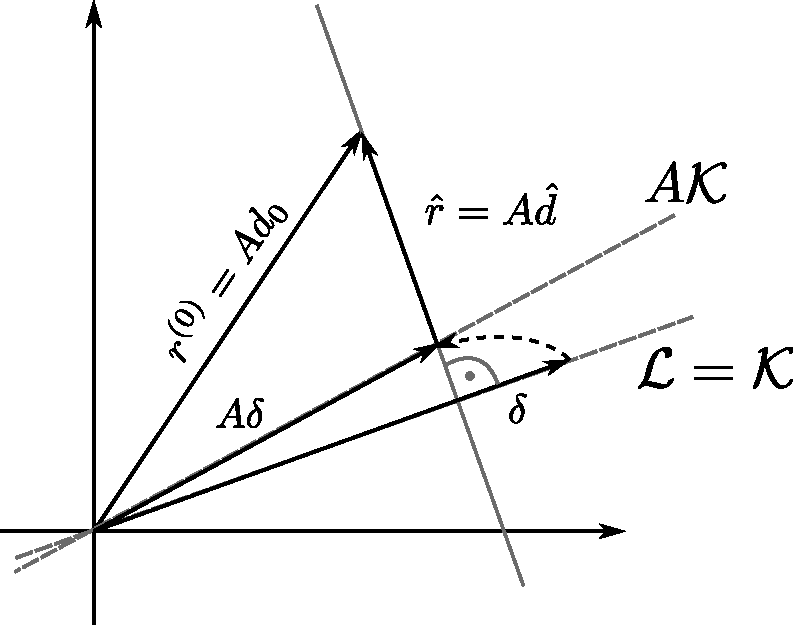
\includegraphics[width=\linewidth]{chapters/2_solvers/2_3_iterative_solvers/figures/projection_orthogonal.pdf}
  \caption{Orthogonal projection process}
  \label{fig:projection_orthogonal}
\end{subfigure}%
\begin{subfigure}{.5\textwidth}
  \centering
  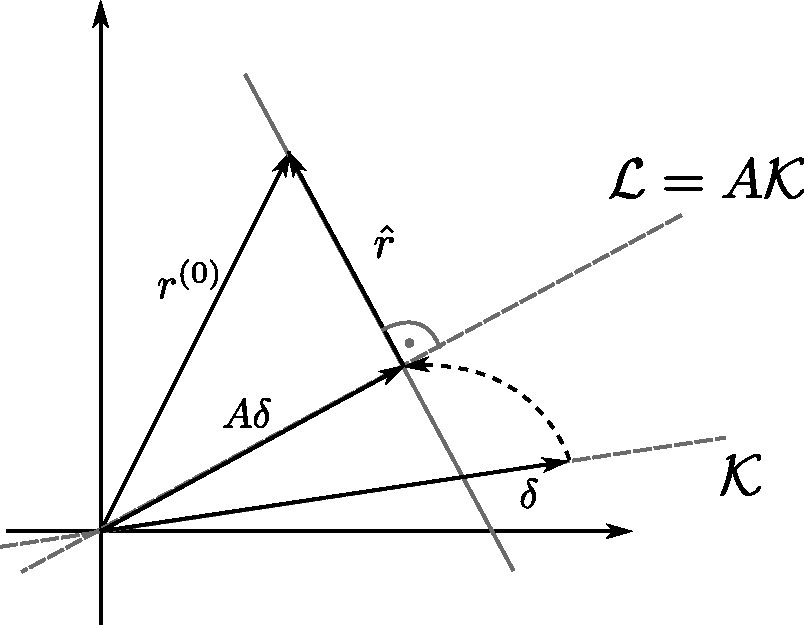
\includegraphics[width=\linewidth]{chapters/2_solvers/2_3_iterative_solvers/figures/projection_oblique.pdf}
  \caption{Oblique projection process}
  \label{fig:projection_oblique}
\end{subfigure}
\caption{Difference between projection methods. Given $\mathcal{K}$ it computes $A\mathcal{K} =A\tilde{\delta}$ with $\tilde{\delta} \in \mathcal{K}$ and then select $\delta$ such that $\iter[0]{r}-A\delta \perp \mathcal{L}$.}
\label{fig:projection}
\end{figure}

\noindent In first case, on the other hand, where $\mathcal{L}=\mathcal{K}$, the orthogonality condition becomes $A\hat{x}-b \perp \mathcal{K}$, which is usually referenced as the Galerkin condition. Figure~\hyperref[fig:projection_oblique]{\ref{fig:projection_oblique}} shows this kind of projection, where the orthogonality is enforced on the projected subspace (thus the name orthogonal projection). In order to analyze its behaviour, let $x^*$ denote the exact solution to the system and $\iter[0]{d}=x^*-\iter[0]{x}$ be the initial error. In a similar fashion, $\hat{d} = x^*-\hat{x}$ is defined with $\hat{x}=\iter[0]{x}+\delta$, which yields the relation:
\begin{equation}
    \hat{r} = A\hat{d} = A(\iter[0]{d}+\delta)
\end{equation}

\noindent The constraint $A\hat{x}-b \perp \mathcal{K}$ can be rewritten as $\iter[0]{r}-A\delta \perp \mathcal{K}$ which leads to:
\begin{equation}
    \langle A(\iter[0]{d}-\delta); w\rangle = 0\text{,}\;\; \forall w \in \mathcal{K}
\end{equation}

\noindent In this formula, $\langle\dots;\dots\rangle$ denotes the inner product and since $A$ is symmetric positive definite. it allows for such an operation $\langle \iter[0]{d}-\delta); w\rangle_A$ (see \cite{saad_iterative_2003}). As a result, the vector $\delta$ is the $A$-orthogonal projection of the initial error $\iter[0]{d}$ onto the subspace $\mathcal{K}$ and the error $\hat{d}$ is decreased in each iteration with respect to the $A$-norm:
\begin{equation}
    \normd{\hat{d}}_A \leq \normd{\iter[0]{d}}_A
\end{equation}

\noindent This type of method is termed \textit{error projection} and in terms of error analysis, it is equivalent to minimizing the backward error of the system (i.e. $\hat{x}$ should be close to $x^*$). On the other hand, residual projection methods try to decrease the forward error of the system (i.e. $A\hat{x}$ being close to $Ax^*=b$), on the other hand try to decrease the forward error, both resulting in a good approximation of $x^*$. A detailed discussion of these error types is available from \cite{higham_accuracy_2002} and will not be discussed here any further. As a consequence of the discussion on projection methods, for the remainder of this thesis it will be assumed that $A$ meets the required characteristics for the selected method (i.e. $A$ is symmetric positive definite whenever $\mathcal{L}=\mathcal{K}$).

\subsubsection{Steepest Descent}
\label{sec:steepest_descent}

The method of steepest descent provides a simple example of an one-dimensional projection process. Such a projection is defined when $v$ and $w$ are two vectors and the subspaces are given by:
\begin{equation}
    \mathcal{K}=span\{v\}\;\; \text{and} \;\; \mathcal{L}=span\{w\}
\end{equation}

\noindent For such a case, the correction term is given by $\delta=\alpha v$, where $\alpha$ is a scalar and the orthogonality condition $r-A\delta \perp w$ results in:
\begin{equation}
    \alpha = \frac{\langle r;w\rangle}{\langle Av;w\rangle}
\end{equation}

\noindent The method consist of taking a step which $v=r$ and $w=r$ (and thus $\mathcal{L}=\mathcal{K}$), which implies that A has to be symmetric positive definite. The whole process is outlined in  Algorithm~\hyperref[alg:steepest_descent]{\ref{alg:steepest_descent}} where $r$ is the negative of the gradient direction in each iteration. As a result, the algorithm takes a step into the direction that yields the fastest rate of decrease \textit{locally}.

\begin{algorithm}[h]
  \caption{Steepest Descent}
  \label{alg:steepest_descent}
  \SetAlgoLined
  \DontPrintSemicolon
  \KwIn{matrix $A \in \mathbb{R}^{n \times n}$, vector $b \in \mathbb{R}^{n}$ and initial solution $\iter[0]{x} \in \mathbb{R}^{n}$}
  \KwOut{approximate solution $\iter[m]{x}$ to the system $Ax=b$\\
  \hrulealg}
  $r = b-A\iter[0]{x}$ \\
  $p = Ar$ \\
  \For{$i = 1$ \KwTo $m$} {
    $\alpha = \langle r;r \rangle / \langle p;r \rangle$ \\
    $\iter[i]{x} = \iter[i-1]{x}+\alpha r$ \\
    $r = r - \alpha p$ \\
    $p = Ar$ \\
  }
\end{algorithm}

\noindent Since the algorithmic interpretation might be quite difficult to understand, the first step of the steepest descent method is illustrated in Figure~\hyperref[fig:steepest_descent]{\ref{fig:steepest_descent}}. The new solution $\iter[1]{x}$ is created by $\iter[1]{x}=\iter[0]{x}+\alpha \iter[0]{r}$, where $\alpha$ is determined so that $\iter[0]{r} \perp \iter[1]{r}$ holds. Because $\hat{r}=A\hat{d}$ and $\hat{d}=x^*-\hat{x}$, each step of the iteration minimizes:
\begin{equation}
f(x) = \norm{x^*-\hat{x}}_A^2 = \langle A(x^*-\hat{x});(x^*-x)\rangle
\end{equation}
\noindent over all the vectors of the form $x+\alpha v$ where $v$ is the negative of the gradient direction $-\nabla f$.

\begin{figure}
\centering
\begin{subfigure}{.5\textwidth}
  \centering
  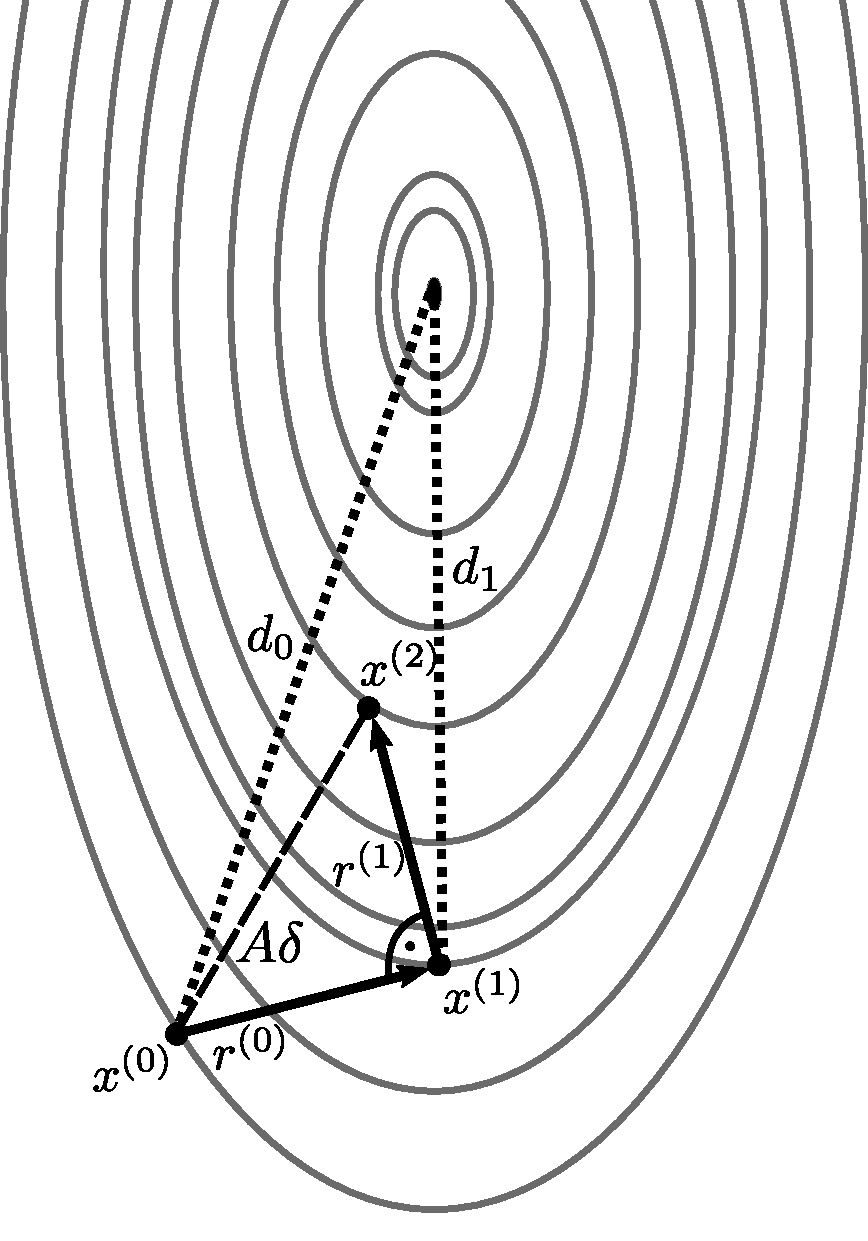
\includegraphics[width=0.9\linewidth]{chapters/2_solvers/2_3_iterative_solvers/figures/steepest_descent.pdf}
  \caption{Steepest Descent}
  \label{fig:steepest_descent}
\end{subfigure}%
\begin{subfigure}{.5\textwidth}
  \centering
  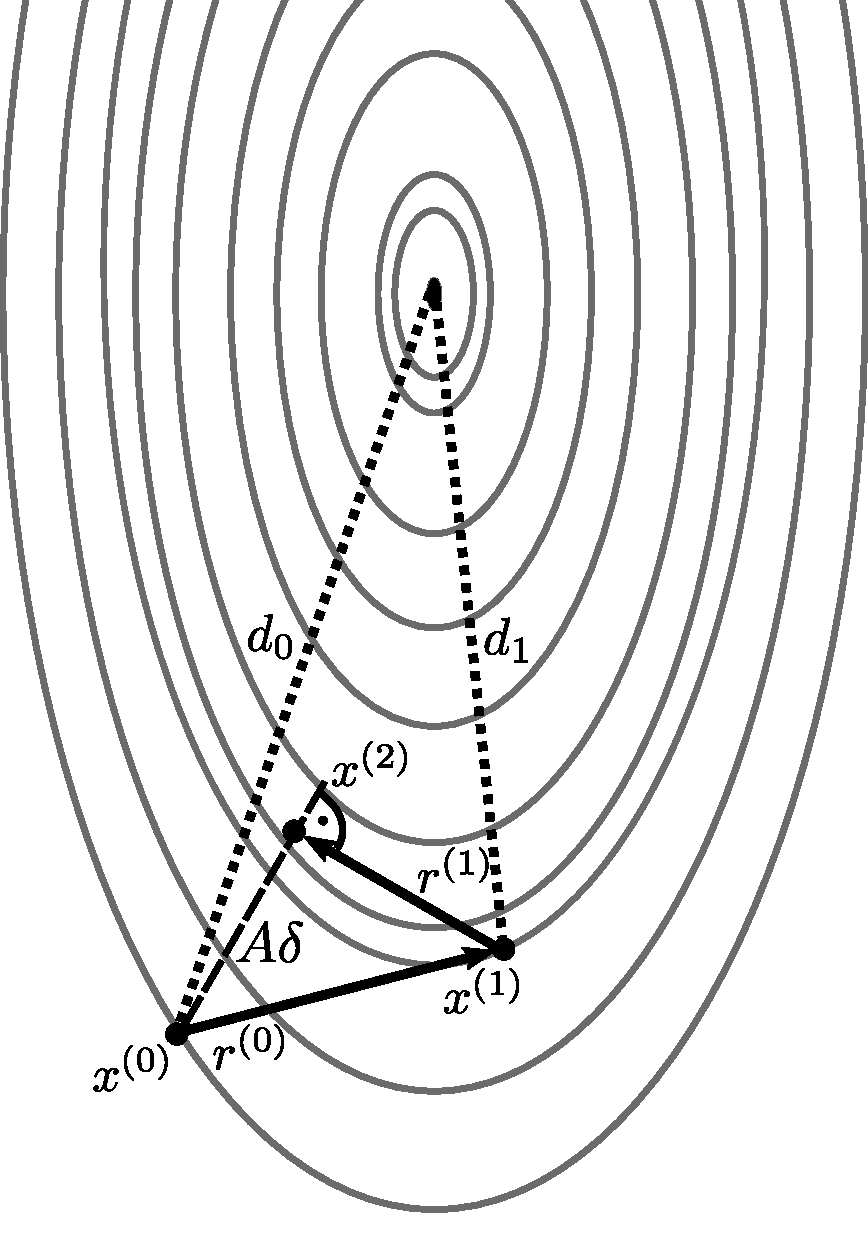
\includegraphics[width=0.9\linewidth]{chapters/2_solvers/2_3_iterative_solvers/figures/mr.pdf}
  \caption{Minimal Residualm}
  \label{fig:mr}
\end{subfigure}
\caption{Comparison of the first iteration of steepest descent and minimal residual method. Steepest descent minimizes $\normd{\hat{d}}_A$ while minimal residual minimizes $\norm{\hat{r}}_2$}
\label{fig:one_d_projections}
\end{figure}


\subsubsection{Minimal Residual (MR)}
\label{sec:mr}
The minimal residual (MR) method is the counterpart to steepest descent for non-symmetric positive definite matrices. Therefore, $\mathcal{L}=A\mathcal{K}$ and as such, it takes a step with $v=r$ and $w=Ar$, giving rise to the procedure written in Algorithm~\hyperref[alg:mr]{\ref{alg:mr}} and the first iteration is depicted in Figure~\hyperref[fig:mr]{\ref{fig:mr}}. Note that in the comparison to steepest descent (shown in Figure~\hyperref[fig:one_d_projections]{\ref{fig:one_d_projections}}, the first iteration leads to a much smaller decrease in the actual error $\hat{d}$, but this does not necessarily hold for all linear systems. Generally speaking, steepest descent optimizes the error more efficiently (and is therefore preferred in the symmetric case), but under very favourable properties of the matrix $A$, MR could converge faster. Thus, the choice of algorithm is actually dependent on the problem that needs to be solved.

Despite that, it has been proven that both methods will converge if the matrix $A$ meets the required conditions (positive definite for both algorithms, symmetric for steepest descent, see \cite{saad_iterative_2003}). The main difference between the two methods is that MR minimizes the norm of the residual $\norm{\hat{r}}_2$ in each iteration in the direction of $r$:
\begin{equation}
    f(x) = \norm{b-A\hat{x}}_2^2    
\end{equation}


\begin{algorithm}[h]
  \caption{Minimal Residual}
  \label{alg:mr}
  \SetAlgoLined
  \DontPrintSemicolon
  \KwIn{matrix $A \in \mathbb{R}^{n \times n}$, vector $b \in \mathbb{R}^{n}$ and initial solution $\iter[0]{x} \in \mathbb{R}^{n}$}
  \KwOut{approximate solution $\iter[m]{x}$ to the system $Ax=b$\\
  \hrulealg}
  $r = b-A\iter[0]{x}$ \\
  $p = Ar$ \\
  \For{$i = 1$ \KwTo $m$} {
    $\alpha = \langle p;r \rangle / \langle p;p \rangle$ \\
    $\iter[i]{x} = \iter[i-1]{x}+\alpha r$ \\
    $r = r - \alpha p$ \\
    $p = Ar$ \\
  }
\end{algorithm}

\noindentAs a final remark in this section, it should be noted that it is quite easy to transform a positive definite matrix $A$ into a symmetric positive matrix by calculating $A+\transp{A}$. Therefore, both algorithms can be used interchangeably and the choice depends on the actual problem at hand. Furthermore, any linear system involving a non-singular matrix $A$ can be turned into a a system with a positive definite matrix by multiplying the system with $\transp{A}$ from the left. Thus, the original equation is replaced by:
\begin{equation}
    \transp{A}Ax = \transp{A}b
\end{equation}

